\documentclass{article}

\usepackage{amsmath}
\usepackage{amssymb}
\usepackage{indentfirst}
\usepackage{enumitem}
\usepackage{bbm}
\usepackage{graphicx}
\usepackage{booktabs}
\usepackage{tikz}
\usepackage[top=1cm, bottom=4cm, left=2cm, right=2cm]{geometry}
\renewcommand{\thesubsection}{\thesection.\alph{subsection}}
\newenvironment{QandA}{\begin{enumerate}}{\end{enumerate}}
\newcommand\supquestion[1]{\item[]\emph{#1}}
\newcommand\question{\item}
\newcommand\answer{\item[\textbf{A:}]}\newcommand{\formfill}{\underline{\hspace{1cm}}}


\usetikzlibrary{shapes.geometric, arrows}
\tikzstyle{startstop} = [rectangle, rounded corners, minimum width=3cm, minimum height=1cm,text centered, draw=black]
\tikzstyle{arrow} = [thick,->,>=stealth]

\begin{document}
\begin{flushleft}
Andrew Yeh \\
Taylor \\
Research Proposal\\
\today{}\\
\end{flushleft}

\section{Research Question}
Does increased repetition of the contract game decrease moral hazard and adverse selection problems?
\subsection{Introduction}
Prior research has studied the role of moral hazard and adverse selection on contract behavior for principal-agent problems. \cite{besterRationing} shows that institutions can use contracts to encourage self-selection, e.g. borrowers for less risky projects put up more collateral for a higher interest rate while borrowers for more risky projects put up less collateral for a lower interest rate. \cite{holmstrom} derives a structure for a contract between principal and agent given imperfect information from the principal to achieve a second-best solution to social welfare. 
\par \cite{besterRationing} and \cite{holmstrom} study single-period, cross-sectional models and find the equilibrium of supply and demand in that single period given utility maximization. In Game Theory, this would correspond to a normal-form game, and the second-best solution found by \cite{holmstrom} corresponds to a Nash Equilibrium. However, contracts may also be periodically renegotiated (``repeating''), and the success and failure of the agent's efforts can have implications for future contracts. For example, bank lending outcomes feed into credit scores so that the history of prior credit actions are encoded into a score that banks can access. In Game Theory, this is known as a repeated game: the contract and agreement is known as a stage game, and the stage game repeats with all participants seeking to maximize their own \emph{total} payoff. 
\par Game Theory states that in repeated games where the stage game repeats, the relevant equilibria is no longer the Nash Equilibrium of the individual stage games but rather a subgame perfect equilibrium (SPE), and that players can undertake strategies to sustain payoff profiles that are not individually Nash Equilibrium in the stage game by threatening a lower-valued Nash Equilibrium, e.g. if the agent slacks with 95\% probability, the principal will fire the agent.
\par I propose testing the idea that repeated games leads to less moral hazard and adverse selection problems in executive compensation contracts by investigating whether firms/board members who have their compensation contracts regularly re-negotiated or tied to performance outcomes (dynamic renegotiation) face fewer moral hazard problems.
\subsection{Constructs and Proxies}
Our hypotheses are related to re-negotiation leading to fewer instances of moral hazard. We use the following constructs and proxies for moral hazard and the cost of moral hazard:
\begin{enumerate}
	\item Fraud
	\subitem The most straightforward proxy for moral hazard is fraudulent behavior by managers that improve their own welfare and decrease the welfare of the principals.
	\item Earnings management
	\subitem Manipulating earnings does not improve the valuation of the firm which is determined by true earnings. Therefore, it does not improve social welfare. However, empirically, earnings management does increase the stock price and so improves the agent's utility.
	\item Fired
	\subitem Whether an executive is fired is an imperfect proxy for the existence of moral hazard. Executives may also be fired for poor performance as well.
	\item Severance package
	\subitem In a repeated game, moral hazard is averted by threatening the agent with being fired (Nash Equilibrium). If being fired is not as costly for the agent, the threat carries less weight. 
	\item Interest coverage ratio
	\subitem Patience is an important factor for determining whether participants deviate from a repeated game's cooperative equilibrium. If patience is low enough, participants may prefer the rewards from a one-shot deviation over the rewards from continual cooperation. The interest coverage ratio is a construct for patience of the CEO and CFO in particular: when interest coverage is low, managers must adopt a short-term perspective to allow the company to survive and have less patience. Though this can be considered either endogeneously (attracting low patience managers) or exogeneously (forcing managers to take a short-term perspective), it will either way have an effect on the discount rate of the agent differential from the risk-neutral principal which then decreases the penalty for moral hazard.
\end{enumerate}
\subsection{Hypotheses}
\begin{enumerate}
	\item Within the same industry, when firms re-negotiate compensation contracts with CEOs frequently, the contracting game approaches a repeated game and...
	\begin{enumerate}
		\item Fraud is less likely.
		\item Earnings management has a lower magnitude.
		\item Executives are less likely to be fired.
	\end{enumerate}
	\item Within the same industry, when severance packages are higher or the interest coverage is lower, there is a lower punishment for moral hazard and...
	\begin{enumerate}
		\item Fraud is more likely.
		\item Earnings management has a higher magnitude.
		\item Executives are more likely to be fired.
	\end{enumerate}
	\item Hypotheses 1 is also true when firms have more pay-for-performance clauses which double as dynamic re-negotiation.
	\item The effects of re-negotiation, severance and patience, and pay-for-performance documented in hypotheses 1-3 are additive to one another.
\end{enumerate}

\section{Theory}
This research question draws from the incentive-compensation, principal-agent, and Game Theory literature. From the principal-agent and incentive-compensation literature, we use the finding that utility maximizing behavior leads to incentive-compensation contracts designed to trade off social welfare and the utility maximization in order to find a Nash Equilibrium. From Game Theory, we use the finding that repeated games allow players to cooperate and maintain an equilibrium strategy that maximizes social welfare. Our research question asks what happens when you combine the theories of the three fields and uses executive compensation as a setting to test hypotheses.

\section{Related Literature}
\par In the contracting literature, \cite{besterRationing} covers how contracts can be used to avoid adverse selection. \cite{holmstrom} covers how contracts can be used to avoid moral hazard.
\par In the game theory literature, \cite{repeatedGames} and many others have shown that SPEs in repeated games often have different payoff profiles than the Nash equilibrium of the stage game.
\par There has been some work on multi-period contracting. \cite{holstromMulti} extends the work of \cite{holmstrom} to multi-period models but without game theoretic strategies. \cite{gameTheoryLoan} examines the application of game theory to whether a borrower (agent) will repay his loan to the bank (principal). \cite{infiniteHazard} and \cite{repeatedHazard} examine moral hazard from an infinitely repeated game perspective and find that repeated games lead to equilibria with a higher social welfare than that found by the \cite{holmstrom} or \cite{besterRationing} single-period models. \cite{lambert_long-term_1983} and \cite{radner_monitoring_1981} find the same or similar results for finitely repeated games and additionally find that the optimal compensation necessarily includes memory: present payoffs must depend on past results. 
\par While there has been theoretical work done in the intersection of contracting theory and game theory, there is a gap in the literature for empirical verification. For example, the above literature is purely theoretical and even past literature on this topic with real-world examples or motivations like \ref{rubinstein_repeated_1983} for moral hazard in insurance are based on theory without verification from empirical evidence. We attempt to extend and test these theoretical findings.

\section{Research Design}
I propose a causal chain linking compensation contract negotiation aspects to a repeated game in Figure \ref{proposed_causal_chain}. I also propose a causal chain that pre-assumes a repeated game structure and links motivations for deviation from a cooperative equilibrium to Moral Hazard in Figure \ref{proposed_causal_chain_2}.

\begin{figure}
\begin{center}
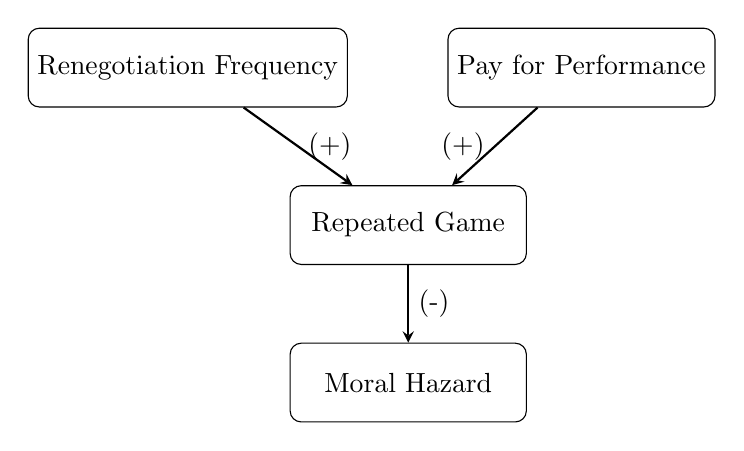
\begin{tikzpicture}[node distance=2cm]
\node (start1) [startstop] {Renegotiation Frequency};
\node (start2) [startstop, right of = start1, xshift = 3cm] {Pay for Performance};
\node (intermediate) [startstop, below of = start2, xshift = -2.2cm] {Repeated Game};
\node (end) [startstop, below of=intermediate] {Moral Hazard};
\draw [arrow] (intermediate) -- node[anchor=west] {(-)} (end);
\draw [arrow] (start1) -- node[anchor=west] {(+)} (intermediate);
\draw [arrow] (start2) -- node[anchor=east] {(+)} (intermediate);
\end{tikzpicture}
\end{center}
\caption{Proposed causal chain}
\label{proposed_causal_chain}
\end{figure}

\begin{figure}
\begin{center}
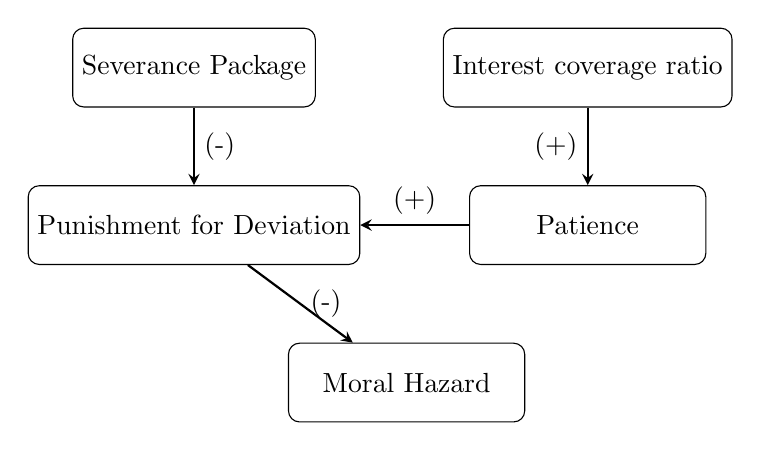
\begin{tikzpicture}[node distance=2cm]
\node (start1) [startstop] {Severance Package};
\node (start2) [startstop, right of = start1, xshift = 3cm] {Interest coverage ratio};
\node (intermediate1) [startstop, below of = start1] {Punishment for Deviation};
\node (intermediate2) [startstop, below of = start2] {Patience};
\node (end) [startstop, below of=intermediate1, xshift = 2.7cm] {Moral Hazard};
\draw [arrow] (intermediate1) -- node[anchor=west] {(-)} (end);
\draw [arrow] (intermediate2) -- node[anchor=south] {(+)} (intermediate1);
\draw [arrow] (start1) -- node[anchor=west] {(-)} (intermediate1);
\draw [arrow] (start2) -- node[anchor=east] {(+)} (intermediate2);
\end{tikzpicture}
\end{center}
\caption{Proposed causal chain, assuming a repeated game structure.}
\label{proposed_causal_chain_2}
\end{figure}

To date, I am not aware of any setting where there is an exogeneous shock to renegotiation frequency, pay-for-performance clauses, or severance packages. While interest coverage ratio may be affected in banks exogeneously via federal regulation, the shocks cannot have as-if-random assignment since it disproportionately affects already highly levered firms.
\par Therefore, I consider a series of alternative, endogeneous explanations and attempt to control or falsify each in turn. Though there may be other alternative explanations not considered making it impossible prove the causal chain, explicitly ruling out the most plausible alternatives at least lends credibility to the proposed hypotheses.
\par For renegotiation and pay for performance:
\begin{enumerate}
	\item More active board of directors renegotiate frequently but also monitor the CEO more closely. The active monitoring is what actually causes the decrease in moral hazard.
	\subitem To address this, I control for board meeting frequency and the board's ownership percentage of the company.
	\item Some CEOs are more amenable to renegotiation and pay for performance clauses than others. The types of CEOs who are more amenable are less likely to commit acts of moral hazard.
	\subitem To address this, I add fixed effects for CEOs in the regression and a control variable for CEO age.
	\item Some industries (time periods) are more amenable to fraud than others. Perhaps the same industries in which fraud is more common happen to be industries where contract renegotiation or pay-for-performance are more common.
	\subitem To address this, I add year fixed effects and run a separate regression for each industry. I separate out industry regressions instead of adding industry-fixed effects in order to estimate a different fixed effect coefficient for each industry, e.g. a different year fixed effect for each industry to capture the industry-year interaction effects.
\end{enumerate}
\par The data is on the firm-quarter level. Altogether:
\begin{align*}
Moral Hazard_i &\sim \alpha + \beta_{i,1} RepeatedGameStructure + \beta_{i,2} Board + \beta_{i,3} CEO + \beta_{i,4} Year\\
Moral Hazard_i &\sim \alpha + \beta_{i,1} Severance + \beta_{i,2} Patience + \beta_{i,3} Board + \beta_{i,4} CEO + \beta_{i,5} Year
\end{align*}
where $i$ denotes the industry subscript for each separate OLS regression and $RepeatedGameStructure$ is either just re-negotiation frequency, just pay-for-performance sensitivtiy, or both features jointly estimated. The effects of severance and patience are measured jointly in the same regression specification since they affect the penalty for deviation simultaneously.

\section{Proposal Limitations}
Contract re-negotiation and pay-for-performance clauses are highly endogeneous and slow moving. Exogeneous shocks to these aspects of compensation rarely affect all firms equally, breaking the as-if-random assignment necessary for natural experiments.
\par Earnings management is an entire area of study for structural modeling and the true value is unobserved by the investor, so constructs for earnings management, e.g. accruals to earnings, used in this research design are proxies instead of the actual value.
\par Getting fired may not be as great a threat to CEOs as envisioned, and the costliness of this threat is both unobserved, heterogeneous, and may be time varying based on the number of alternative opportunities either as CEO or otherwise at other companies.

\bibliographystyle{plain} % We choose the "plain" reference style
\bibliography{refs} % Entries are in the refs.bib file


\end{document}